\documentclass[12pt,a4paper]{article}

\usepackage[left=1.5cm,top=1cm,right=1.5cm,bottom=60pt]{geometry}
\usepackage[utf8]{inputenc}
\usepackage[spanish]{babel}
\usepackage{amsmath,amssymb ,amsfonts,xcolor,tikz}
\usepackage{multicol}
\usepackage[shortlabels]{enumitem}
\usepackage{eso-pic}
\usetikzlibrary{calc}
\usepackage{framed}

\definecolor{oroUnam}{rgb}{0.835, 0.624, 0.0588}
\definecolor{azulUnam}{rgb}{0, 0.24, 0.47}
\definecolor{gris}{RGB}{195, 195, 195}

\newcommand{\sect}[1]{
	\begin{tcolorbox}[colframe= white,top=2pt, bottom=2pt, colback = gris]
	 \textbf{#1} %\centering
    \end{tcolorbox}
 }

\setlength{\columnsep}{30pt}
\setlength{\columnseprule}{0.2pt}
\setlength{\parindent}{0pt}%


\usepackage[most]{tcolorbox}

\newtcolorbox[auto counter ]{Exercice}[1][]{
    enhanced,left=0pt,top=8pt,frame hidden,bottom=0pt,before upper={\hspace*{1cm}},
    colback=white,
    interior code app= {\node[fill=gris, anchor=west,text width=0.5cm,text badly centered]at ([shift={(0.1,-0.5)}]frame.north west){{\large\color{white} \textbf{\centering\thetcbcounter}}};},nobeforeafter}



\begin{document}

\begin{tikzpicture}[remember picture,overlay]

\node[fill=gris,
rectangle,
text width = 5cm,
anchor= west, 
inner xsep= 0.5cm, inner ysep=0.3cm](A) at([shift={(0.99,-1)}]current page.north west){{\Large \textbf{\sffamily\color{white} Hoja de ejercicios }}};  

\end{tikzpicture}


\begin{tikzpicture}[remember picture, overlay]
	
	% Barra azul 

	\fill[azulUnam] (current page.north west)rectangle([shift={(1,0)}]current page.south west);
	
	\draw[line width= 3.8pt,oroUnam] ($(A.north west)!9!(A.south west)$ )--++(-2.5,0) ;
	
	\draw[line width= 3.8pt,oroUnam] ($(A.north west)!18!(A.south west)$ )--++(-2.5,0) ;
	
	% MATEM\'ATICAS PARA EL LABORATORIO
	
	\node[white,rotate=90] at([shift={(0.5,-5.33)}]current page.north west){{\Large \textbf{\sffamily Matem\'aticas para el laboratorio}}};
	
	% ECOFISIOLOG\'IA
	
	\node[white,rotate=90] at([shift={(0.5,-15.66)}]current page.north west){{\Large \textbf{\sffamily Ecofisiolog\'ia}}};
	
	% DR. ALVARO BARRETO
	
	\node[white,rotate=90] at([shift={(0.5,-25)}]current page.north west){{\Large \textbf{\sffamily Dr. Alvaro Barreto}}};   

\end{tikzpicture}

El ejercicio consiste en determinar la cantidad de cada reactivo que se debe de preparar para realizar las t\'ecnicas de an\'alisis enzim\'atico que se describen a continuaci\'on:

\begin{multicols}{2}

    \raggedcolumns
    
\sect{Un poco de contexto}

Supongamos que muy pronto finalizar\'a un experimento que tiene por objetivo determinar la influencia de la salinidad (3, 15, y 35 g/L) en la fisiolog\'ia digestiva del robalo blanco \textit{Centropomus undecimalis}. Por lo tanto, se necesita medir la actividad enzim\'atica del est\'omago, ciego e intestino (ver figura~\ref{fig:ejercicio}). 

\sect{An\'alisis de actividad enzim\'atica}

\begin{Exercice}\textbf{ Preparaci\'on de homogenizados}

	Se tomar\'an nueve organismos por cada tratamiento (tres por replica), después de proceder con la eutanasia se va retirar el est\'omago, ciego e intestino, los cuales se van a triturar en nitr\'ogeno l\'iquido y se almacenar\'a en tubos de 10 mL a una temperatura de -80 $^\circ$C. Para obtener el extracto enzim\'atico, se va agregar buffer glicina-HCl 0.1 M a pH 3 al estómago y Tris-HCl 30 mM + CaCl$_2$ 12.5 mM pH 7.5 al ciego e intestino en una dilución de 1:5 y 1:2 respectivamente (suponga que utilizar\'a dos gramos de tejido).
	
	Despu\'es de agregar el buffer los extractos se homogenizar\'an con un ULTRA TURRAX$^{\mbox{\scriptsize\textregistered}}$  IKA T18 Basic durante 15 segundos en cada muestra, siempre en frío. Posteriormente se va ha centrifugar a 12,000 rpm a una temperatura de 4$^\circ$C por 20 minutos, al final se va retirar el sobrenadante y colocar en microtubos de 1.5 mL, los cuales se van a congelar en nitrógeno líquido y almacenar a una temperatura de -80 $^\circ$C para posteriormente ser utilizados. 
	
\end{Exercice}
    
\begin{Exercice} \textbf{Proteasas ácidas}
	
	Para determinar la actividad se utilizar\'a la técnica de Anson (1938), en 1 mL de hemoglobina al 1\% en tampón glicina-HCl 0.1 M a pH 2. Se va a\~nadir 5 $\mu$l del extracto multienzimático y se incubar\'a durante 5 minutos a 37°C. Para detener la reacción se le adicionar\'a 0.5 mL de ácido tricloro acético (TCA) al 20\%. Después se dejar\'a reposar la mezcla de reacción 15 minutos a 4$^\circ$C, posteriormente se va centrifugar a 12,000 rpm durante 5 minutos, y se retirar\'a el sobrenadante para medir la actividad. La actividad se definir\'a como 1 $\mu$g de tirosina hidrolizada por minuto. Usando como coeficiente de extinción molar de 0.008 a 280 nm.

\end{Exercice}

\begin{Exercice} \textbf{Proteasas alcalinas}
	
	Se utilizar\'a el método de Kunitz (1947) modificado por Walker (1984), usando como sustrato caseína al 1\% en tampón 100 mM Tris-HCl + 10 mM CaCl$_2$ a pH 9. Se le agregar\'a 0.5 mL de caseína, más 0.5 mL de tampón Tris-HCl 100 mM + CaCl$_2$ 10 mM a pH 9 y 10 $\mu$L de extracto enzimático, se incubar\'a por 10 minutos a 25 $^\circ$C, posteriormente la reacción se detendr\'a con 0.5 mL de \'acido tricloroacético (TCA) al 20\%, se centrifugar\'a a 12,000 rpm por 5 minutos, la actividad se definir\'a de acuerdo al apartado anterior.

\end{Exercice}

\begin{Exercice}\textbf{Tripsina}
	
	Se utilizar\'a el método de Erlanger et al. (1961), usando como sustrato BAPNA (N-$\alpha$- benzoil-DL-arginina 4-nitroanilida) al 3.5 mM en buffer 50 mM Tris-HCl + 10 mM CaCl$_2$ a pH 8, el BAPNA se diluir\'a previamente en 200 $\mu$L de DMSO. Para iniciar la reacción se mezclar\'a 990 $\mu$L del sustrato con 10 $\mu$L del extracto enzimático y se incubar\'a por 30 minutos a 25 $^\circ$C. La reacción se detendr\'a adicionando 250 $\mu$L de TCA al 20\%, se centrifugar\'a a 12,000 rpm por 5 minutos. La actividad se definir\'a de acuerdo a Dimes et al. (1994), como 1 $\mu$mol de p-nitroanilida hidrolizada por minuto, usando como coeficiente de extinción molar 8.2 a 410 nm.
	
\end{Exercice}

\begin{Exercice} \textbf{Quimotripsina}
	
	Se determinar\'a por el método de Lainé et al. (1993), utilizando como sustrato Suc-AAFP-pNA (N-succinyl-alanine-alanine-proline-phenylalanine-p-nitroanilide) al 1mM disuelto en DMSO. Para iniciar la reacción se agregar\'a en una celda de cuarzo 960 $\mu$L de buffer Tris 0.1 M a pH 8 y 10 $\mu$L de Suc-AAFP-pNA, despu\'es de esto se le agregar\'a 20 $\mu$L del extracto, se agitar\'a y medir\'a su absorbancia en el minuto uno y dos a 405 nm. La actividad se definir\'a como 1 $\mu$mol de p-nitroanilida hidrolizada entre el minuto uno y dos, usando como coeficiente de extinción molar 8.2 a 405 nm.
	
\end{Exercice}

\begin{Exercice}\textbf{Peso molecular (g/M) de reactivos disponibles en el laboratorio}
	\begin{enumerate}[1)]
		\item Tris-HCL: 157.6 
		\item Tris: 121.14 
		\item Glicina-HCl: 111.53
		\item CaCl$_2$ $\centerdot$ 2H$_2$O: 147.01
		\item Hemoglobina: 54,500
		\item TCA: 163.39
		\item Case\'ina: 23,983
		\item BAPNA: 434.88
		\item Suc-AAFP-pNA: 451.43
		\item DMSO (es un solvente): 78.13
		\item Agua: 18.02 g/mol
	\end{enumerate}
\end{Exercice}

\end{multicols}

\begin{figure}[h]
	\begin{leftbar}
		
		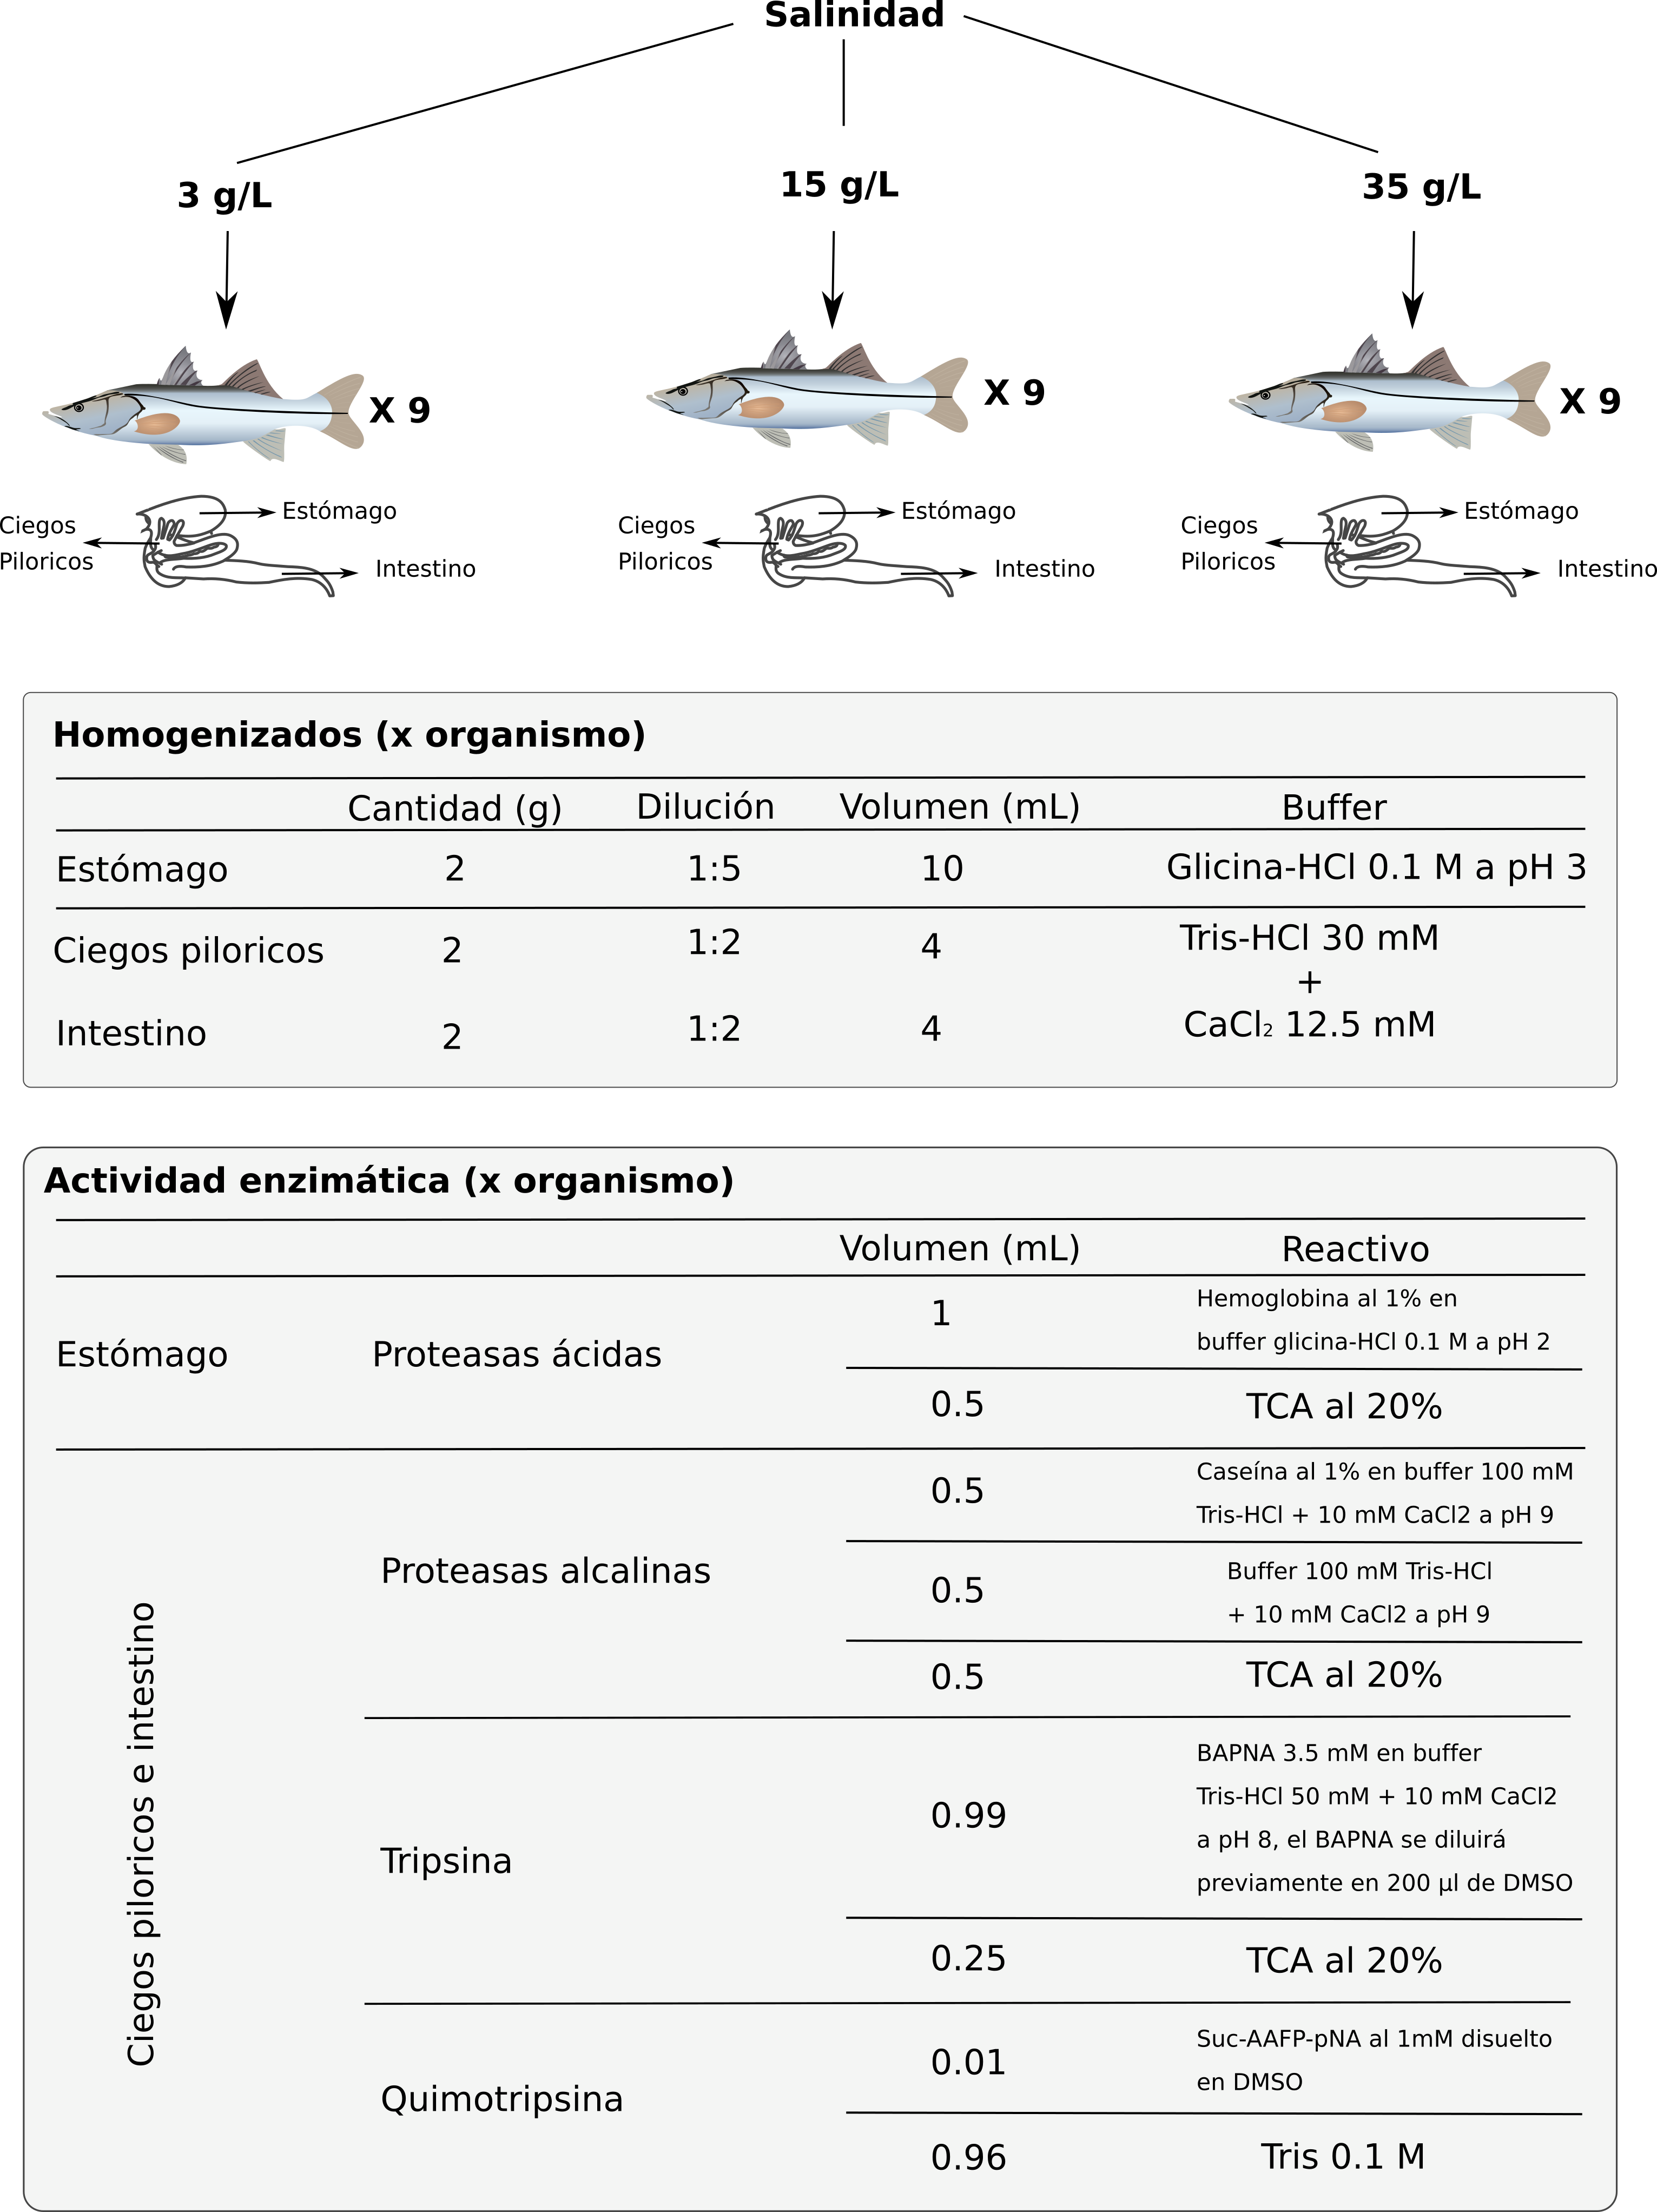
\includegraphics[width=\textwidth]{ejercicio.png}
		\centering
		\caption{\textit{Diagrama del an\'alisis de actividad enzim\'atica del robalo blanco \textit{Centropomus undecimalis} cultivados en salinidades de 3, 15, y 35 g/L.}}
		\label{fig:ejercicio}
		
	\end{leftbar}
	
\end{figure}

\end{document} 